\documentclass[9pt,twoside,lineno]{pnas-new}

\usepackage{longtable}
\usepackage{booktabs}


\templatetype{pnassupportinginfo}
%\AtBeginEnvironment{longtable}{\ssfamily}



\title{Deconstructing the gender gap in chess ratings}

\author{Wei Ji Ma, Nikos I. Bosse, Jose Camacho-Collados, Richard L. Smith, Gy\"orgy Barab\'as, David Smerdon, Yifan Hou}

\correspondingauthor{Wei Ji Ma.\\E-mail: weijima@nyu.edu}

\begin{document}

\maketitle
\SItext
\section*{The negative hypergeometric distribution and Knapp's test}
\medskip

Suppose, within a single federation or overall, there are $M$ men, $W$ women, and the $K$'th best woman is ranked $R$ overall. In the following discussion, we treat $M,\ W$ and $K$ as fixed, and $R$ as a random variable.

Under the null hypothesis that the ranking order is random, the probability that $R$ is equal to some value $r$ is given by the probability mass function of the negative hypergeometric distribution \cite{knapp2010prsb}:
\begin{equation}
  \Pr(R = r)
  = \frac{\binom{r - 1}{K - 1}
  \binom{W + M - r}{W - K}}{\binom{W + M}{W}} ,
  \label{eq:KT1}
\end{equation}
provided $K \le r \le M + K$. If the observed rank is $R=R^*$, then the probability $f$ of a result equal to or more extreme than that observed is 
\begin{equation}
  f = \sum_{r=R^*}^{M+K} \Pr(R = r) .
  \label{eq:KT2}
\end{equation}
This is also equivalent to one minus the cumulative distribution function of the negative hypergeometric distribution, evaluated at $r - 1$. Like in the main text, we convert $f$ into a two-sided $p$-value via the standard transformation
\begin{equation}
  p = 2\min(f, 1-f) .
  \label{eq:ptrans}
\end{equation}

Focusing on the top-ranked woman player, we computed \eqref{eq:ptrans} for each federation as well as for the aggregated global rating list, for all 12 data filters (ranging from including all players to including only active non-junior players rated at least 1600). For example, in the complete rating list including juniors but excluding inactive players, we have $W = 17,286$, $M = 153,454$, and if $K=1$ then $R^*=79$ corresponds to Hou Yifan's rank as the top woman player. Evaluating \eqref{eq:ptrans} in this case, $p = 4.8\times 10^{-4}$. As in our main analyses, the $p$-values increase with stricter data filters. When excluding junior, inactive, and lower-rated players, we get $p = 0.066$ (when players rated below 1400 are excluded) or $p = 0.080$ (when players rated below 1600 are excluded). All global results can be seen together in Table~\ref{tab:knapp-global}.

\begin{table}[!ht]
\centering
\caption{Results of applying Knapp's rank analysis to global chess rating data. The first three columns are various data filters; $K$ is the rank of the woman player we focus on ($K = 1$ means the top-rated and $K = 10$ the 10th highest-rated woman); the next two columns are the number of women and men in the data after applying the filters; and the last column is the $p$-value as calculated from \eqref{eq:ptrans}. Results for $K = 1$ and $K = 10$ are visually separated with a small vertical gap in the table.}
\label{tab:knapp-global}
\begin{tabular}[t]{llrrrrr}
\toprule
Juniors & Inactives & Rating floor & K & Women & Men & p-value\\
\midrule
Yes & No & 1000 & 1 & 17286 & 153454 & 0.0005\\
Yes & No & 1400 & 1 & 8293 & 113076 & 0.0080\\
Yes & No & 1600 & 1 & 5306 & 86055 & 0.0188\\
Yes & Yes & 1000 & 1 & 36401 & 307078 & 0.0017\\
Yes & Yes & 1400 & 1 & 20603 & 233274 & 0.0097\\
Yes & Yes & 1600 & 1 & 13894 & 181478 & 0.0192\\
No & Yes & 1000 & 1 & 18200 & 231803 & 0.0214\\
No & Yes & 1400 & 1 & 14638 & 201651 & 0.0298\\
No & Yes & 1600 & 1 & 11180 & 164672 & 0.0388\\
No & No & 1000 & 1 & 5826 & 107497 & 0.0381\\
No & No & 1400 & 1 & 4299 & 92417 & 0.0660\\
No & No & 1600 & 1 & 3236 & 73934 & 0.0804\\
\addlinespace
Yes & No & 1000 & 10 & 17286 & 153454 & < 10\textsuperscript{-4}\\
Yes & No & 1400 & 10 & 8293 & 113076 & < 10\textsuperscript{-4}\\
Yes & No & 1600 & 10 & 5306 & 86055 & < 10\textsuperscript{-4}\\
Yes & Yes & 1000 & 10 & 36401 & 307078 & < 10\textsuperscript{-4}\\
Yes & Yes & 1400 & 10 & 20603 & 233274 & < 10\textsuperscript{-4}\\
Yes & Yes & 1600 & 10 & 13894 & 181478 & < 10\textsuperscript{-4}\\
No & Yes & 1000 & 10 & 18200 & 231803 & < 10\textsuperscript{-4}\\
No & Yes & 1400 & 10 & 14638 & 201651 & < 10\textsuperscript{-4}\\
No & Yes & 1600 & 10 & 11180 & 164672 & < 10\textsuperscript{-4}\\
No & No & 1000 & 10 & 5826 & 107497 & < 10\textsuperscript{-4}\\
No & No & 1400 & 10 & 4299 & 92417 & 0.0001\\
No & No & 1600 & 10 & 3236 & 73934 & 0.0002\\
\bottomrule
\end{tabular}
\end{table}

Still for top-ranked women but disaggregating the data by federations, the results are very similar to what we have obtained for the global top 1 gap in the main text. When retaining all except inactive players, 35 out of the 79 federations with at least 30-30 players of each gender have significantly higher-ranked men, with just one federation (Lithuania) with a significantly higher-ranked top woman than expected by chance. This discrepancy gradually melts away as junior and lower-rated players are excluded, culminating in no significant results out of 30 federations when players who are inactive, junior, or rated below 1600 are excluded.

\begin{table}[!ht]
\centering
\caption{Results of applying Knapp's rank analysis to chess rating data disaggregated by individual federations. The first four columns are as in Table~\ref{tab:knapp-global}; ``Federations'' is the number of federations with at least 30-30 players of each gender after applying the data filters; the final two columns are the number of federations out of these in which women, resp.~men, are significantly higher-ranked than expected by chance (with a significance threshold of 0.05 and after false discovery rate correction to the p-values of the federations within each row). For women, the three-letter labels of the federations with a significant result are also shown (LTU: Lithuania; SVK: Slovakia).}
\label{tab:knapp-per-fed}
\begin{tabular}[t]{llrrrlr}
\toprule
Juniors & Inactives & Rating floor & K & Federations & Women stronger & Men stronger\\
\midrule
Yes & No & 1000 & 1 & 79 & 1 (LTU) & 35\\
Yes & No & 1400 & 1 & 58 & 1 (LTU) & 16\\
Yes & No & 1600 & 1 & 45 & 1 (LTU) & 9\\
Yes & Yes & 1000 & 1 & 99 & 1 (LTU) & 65\\
Yes & Yes & 1400 & 1 & 79 & 1 (LTU) & 38\\
Yes & Yes & 1600 & 1 & 65 & 1 (LTU) & 30\\
No & Yes & 1000 & 1 & 77 & 1 (LTU) & 39\\
No & Yes & 1400 & 1 & 69 & 1 (LTU) & 26\\
No & Yes & 1600 & 1 & 62 & 1 (LTU) & 24\\
No & No & 1000 & 1 & 46 & 1 (LTU) & 10\\
No & No & 1400 & 1 & 40 & 1 (LTU) & 4\\
No & No & 1600 & 1 & 30 & 0 & 0\\
\addlinespace
Yes & No & 1000 & 10 & 79 & 0 & 54\\
Yes & No & 1400 & 10 & 58 & 0 & 18\\
Yes & No & 1600 & 10 & 45 & 0 & 11\\
Yes & Yes & 1000 & 10 & 99 & 0 & 84\\
Yes & Yes & 1400 & 10 & 79 & 0 & 56\\
Yes & Yes & 1600 & 10 & 65 & 0 & 45\\
No & Yes & 1000 & 10 & 77 & 0 & 57\\
No & Yes & 1400 & 10 & 69 & 0 & 45\\
No & Yes & 1600 & 10 & 62 & 0 & 34\\
No & No & 1000 & 10 & 46 & 0 & 12\\
No & No & 1400 & 10 & 40 & 1 (SVK) & 7\\
No & No & 1600 & 10 & 30 & 1 (SVK) & 6\\
\bottomrule
\end{tabular}
\end{table}

We have also repeated the same analysis for the 10th highest-rated woman instead of the top-rated one. The results are also in Tables~\ref{tab:knapp-global}-\ref{tab:knapp-per-fed}.

In summary, Knapp's rank analysis yields results that are consistent with our permutation approach. This gives further confidence that the results are robust.

%We computed \eqref{eq:KT2} for each federation as well as for the complete rating list. For example, in the complete rating list including juniors but excluding inactive players, we have $N=155368$, $M=17389$, and if $K=1$ then $R^*=79$ corresponding to Hou Yifan's rank as the top female player. Evaluating Eqs.~(\ref{eq:KT1})-(\ref{eq:KT2}) in this case, $\Pr(R\ge 79)\approx 0.00025$ which we then interpret as the one-sided p-value under the participation rate hypothesis. When we repeat this analysis (with $K=1$) for the 79 individual federations, we find a statistically significant result ($p<0.05$) in 56 federations, going up to 65 or 64 respectively if $K=10$ or $K=30$ (recall that the criterion for a federation being included is that it should have at least 30 female players). If instead we base the calculation on two-sided p-values, the numbers of statistically significant results are respectively 51, 58, 59 for $K=1,\ 10,\ 30$. However interpreted, these results show that the participation rate hypothesis is rejected for the vast majority of federations. This test is effectively equivalent to Knapp's test \cite{knapp2010prsb} and has the merit of being an exact calculation instead of requiring simulation.



\section*{Global and per-federation permutation results, for all data filters and metrics}

The best way to view the data is to use the interactive application provided as a supplement. It can be downloaded from the public GitHub repository \url{https://github.com/weijima/gender-gap-chess}. To run the application locally, open \texttt{/app/app.R} in RStudio and click on the ``Run App'' button (for this to work, all other files in the \texttt{/app} folder must also be downloaded and placed in the same subdirectory). This application is also deployed online at \url{https://dysordys.shinyapps.io/gender-gap-chess/}, and can simply be used from a browser. It will be maintained and kept there for at least one year after publication.

Though not in an interactive form, the global rating data and permutation results are also given here, in Table~\ref{tab:global-perm-SI}. We do not do the same for the per-federation analyses, as that would take over 20 pages even in heavily condensed form. Instead, they are available either from the \texttt{/data} folder of the above GitHub repository, or from the interactive application.

\begin{table}
\caption{\label{tab:global-perm-SI}Results for the global chess rating dataset. The first four columns are the metric and various data filters; ``Observed'' is the observed value of the metric (men minus women); `Permutation'' is the mean plus/minus one standard deviation of the one million permutation samples; and ``p-value'' is computed to four decimal precision via \eqref{eq:ptrans} (where $f$ is the number of permutation samples that are less than the observed value), with a parenthetical W or M in case the result is significant at the 0.05 level favoring either women (W) or men (M).}
\centering
\begin{tabular}[t]{llllrrr}
\toprule
Metric & Juniors & Inactives & Rating floor & Observed & Permutation & p-value\\
\midrule
Overall mean gap & Yes & No & 1000 & 206.7 & -0.0 $\pm$ 2.8 & < 10\textsuperscript{-4} (M)\\
Overall mean gap & Yes & No & 1400 & 78.1 & 0.0 $\pm$ 2.9 & < 10\textsuperscript{-4} (M)\\
Overall mean gap & Yes & No & 1600 & 38.9 & -0.0 $\pm$ 3.0 & < 10\textsuperscript{-4} (M)\\
Overall mean gap & Yes & Yes & 1000 & 169.2 & -0.0 $\pm$ 1.9 & < 10\textsuperscript{-4} (M)\\
Overall mean gap & Yes & Yes & 1400 & 72.9 & -0.0 $\pm$ 1.8 & < 10\textsuperscript{-4} (M)\\
Overall mean gap & Yes & Yes & 1600 & 41.1 & -0.0 $\pm$ 1.8 & < 10\textsuperscript{-4} (M)\\
Overall mean gap & No & Yes & 1000 & 79.2 & 0.0 $\pm$ 2.4 & < 10\textsuperscript{-4} (M)\\
Overall mean gap & No & Yes & 1400 & 45.0 & -0.0 $\pm$ 2.1 & < 10\textsuperscript{-4} (M)\\
Overall mean gap & No & Yes & 1600 & 29.0 & -0.0 $\pm$ 2.0 & < 10\textsuperscript{-4} (M)\\
Overall mean gap & No & No & 1000 & 101.0 & -0.0 $\pm$ 4.3 & < 10\textsuperscript{-4} (M)\\
Overall mean gap & No & No & 1400 & 26.8 & 0.0 $\pm$ 4.0 & < 10\textsuperscript{-4} (M)\\
Overall mean gap & No & No & 1600 & 7.8 & 0.0 $\pm$ 3.8 & 0.0416 (M)\\
\addlinespace
Overall median gap & Yes & No & 1000 & 280.0 & -0.1 $\pm$ 4.1 & < 10\textsuperscript{-4} (M)\\
Overall median gap & Yes & No & 1400 & 100.0 & -0.1 $\pm$ 4.3 & < 10\textsuperscript{-4} (M)\\
Overall median gap & Yes & No & 1600 & 45.5 & -0.0 $\pm$ 4.2 & < 10\textsuperscript{-4} (M)\\
Overall median gap & Yes & Yes & 1000 & 228.0 & 0.1 $\pm$ 2.9 & < 10\textsuperscript{-4} (M)\\
Overall median gap & Yes & Yes & 1400 & 90.0 & -0.0 $\pm$ 3.0 & < 10\textsuperscript{-4} (M)\\
Overall median gap & Yes & Yes & 1600 & 42.5 & -0.1 $\pm$ 2.6 & < 10\textsuperscript{-4} (M)\\
Overall median gap & No & Yes & 1000 & 83.0 & -0.1 $\pm$ 3.5 & < 10\textsuperscript{-4} (M)\\
Overall median gap & No & Yes & 1400 & 50.0 & 0.2 $\pm$ 3.1 & < 10\textsuperscript{-4} (M)\\
Overall median gap & No & Yes & 1600 & 24.0 & 0.2 $\pm$ 3.0 & < 10\textsuperscript{-4} (M)\\
Overall median gap & No & No & 1000 & 106.0 & -0.0 $\pm$ 5.7 & < 10\textsuperscript{-4} (M)\\
Overall median gap & No & No & 1400 & 32.0 & -0.1 $\pm$ 5.7 & < 10\textsuperscript{-4} (M)\\
Overall median gap & No & No & 1600 & 8.0 & 0.0 $\pm$ 5.5 & 0.1784\\
\addlinespace
Top 10 gap & Yes & No & 1000 & 229.1 & 88.7 $\pm$ 22.3 & < 10\textsuperscript{-4} (M)\\
Top 10 gap & Yes & No & 1400 & 229.1 & 109.8 $\pm$ 23.0 & < 10\textsuperscript{-4} (M)\\
Top 10 gap & Yes & No & 1600 & 229.1 & 118.7 $\pm$ 23.3 & < 10\textsuperscript{-4} (M)\\
Top 10 gap & Yes & Yes & 1000 & 208.7 & 88.8 $\pm$ 22.5 & < 10\textsuperscript{-4} (M)\\
Top 10 gap & Yes & Yes & 1400 & 208.7 & 102.9 $\pm$ 22.7 & < 10\textsuperscript{-4} (M)\\
Top 10 gap & Yes & Yes & 1600 & 208.7 & 109.8 $\pm$ 22.8 & < 10\textsuperscript{-4} (M)\\
Top 10 gap & No & Yes & 1000 & 208.7 & 110.5 $\pm$ 23.1 & < 10\textsuperscript{-4} (M)\\
Top 10 gap & No & Yes & 1400 & 208.7 & 114.4 $\pm$ 23.2 & < 10\textsuperscript{-4} (M)\\
Top 10 gap & No & Yes & 1600 & 208.7 & 117.9 $\pm$ 23.2 & < 10\textsuperscript{-4} (M)\\
Top 10 gap & No & No & 1000 & 229.1 & 128.0 $\pm$ 23.9 & < 10\textsuperscript{-4} (M)\\
Top 10 gap & No & No & 1400 & 229.1 & 136.4 $\pm$ 24.1 & 0.0000 (M)\\
Top 10 gap & No & No & 1600 & 229.1 & 139.7 $\pm$ 24.3 & 0.0002 (M)\\
\addlinespace
Top 1 gap & Yes & No & 1000 & 208.0 & 87.3 $\pm$ 54.3 & 0.0005 (M)\\
Top 1 gap & Yes & No & 1400 & 208.0 & 103.5 $\pm$ 53.5 & 0.0080 (M)\\
Top 1 gap & Yes & No & 1600 & 208.0 & 110.3 $\pm$ 53.6 & 0.0187 (M)\\
Top 1 gap & Yes & Yes & 1000 & 197.0 & 81.5 $\pm$ 53.6 & 0.0017 (M)\\
Top 1 gap & Yes & Yes & 1400 & 197.0 & 92.7 $\pm$ 53.3 & 0.0097 (M)\\
Top 1 gap & Yes & Yes & 1600 & 197.0 & 98.4 $\pm$ 53.4 & 0.0193 (M)\\
Top 1 gap & No & Yes & 1000 & 197.0 & 97.8 $\pm$ 53.9 & 0.0215 (M)\\
Top 1 gap & No & Yes & 1400 & 197.0 & 100.9 $\pm$ 54.1 & 0.0302 (M)\\
Top 1 gap & No & Yes & 1600 & 197.0 & 103.6 $\pm$ 54.2 & 0.0386 (M)\\
Top 1 gap & No & No & 1000 & 208.0 & 116.4 $\pm$ 54.7 & 0.0383 (M)\\
Top 1 gap & No & No & 1400 & 208.0 & 122.9 $\pm$ 55.4 & 0.0657\\
Top 1 gap & No & No & 1600 & 208.0 & 125.7 $\pm$ 55.7 & 0.0810\\
\addlinespace
Gap in standard deviation & Yes & No & 1000 & 15.5 & 0.0 $\pm$ 1.6 & < 10\textsuperscript{-4} (M)\\
Gap in standard deviation & Yes & No & 1400 & 11.1 & 0.0 $\pm$ 1.9 & < 10\textsuperscript{-4} (M)\\
Gap in standard deviation & Yes & No & 1600 & 12.4 & 0.0 $\pm$ 2.1 & < 10\textsuperscript{-4} (M)\\
Gap in standard deviation & Yes & Yes & 1000 & 6.8 & 0.0 $\pm$ 1.0 & < 10\textsuperscript{-4} (M)\\
Gap in standard deviation & Yes & Yes & 1400 & 14.3 & 0.0 $\pm$ 1.1 & < 10\textsuperscript{-4} (M)\\
Gap in standard deviation & Yes & Yes & 1600 & 18.6 & 0.0 $\pm$ 1.2 & < 10\textsuperscript{-4} (M)\\
Gap in standard deviation & No & Yes & 1000 & -5.0 & 0.0 $\pm$ 1.5 & 0.0006 (W)\\
Gap in standard deviation & No & Yes & 1400 & 12.5 & 0.0 $\pm$ 1.3 & < 10\textsuperscript{-4} (M)\\
Gap in standard deviation & No & Yes & 1600 & 18.4 & -0.0 $\pm$ 1.3 & < 10\textsuperscript{-4} (M)\\
Gap in standard deviation & No & No & 1000 & -32.7 & 0.0 $\pm$ 2.7 & < 10\textsuperscript{-4} (W)\\
Gap in standard deviation & No & No & 1400 & -0.5 & 0.0 $\pm$ 2.5 & 0.8339\\
Gap in standard deviation & No & No & 1600 & 6.0 & 0.0 $\pm$ 2.7 & 0.0263 (M)\\
\bottomrule
\end{tabular}
\end{table}



\section*{Supplementary figures}

Figs.~\ref{fig:age-exp-juniors-noinactives-1400}-\ref{fig:age-exp-nojuniors-noinactives-1600} are structured in the same way as Fig.~3 in the main text, but for the other 11 data filters.

\begin{figure*}[p]
  \centering
  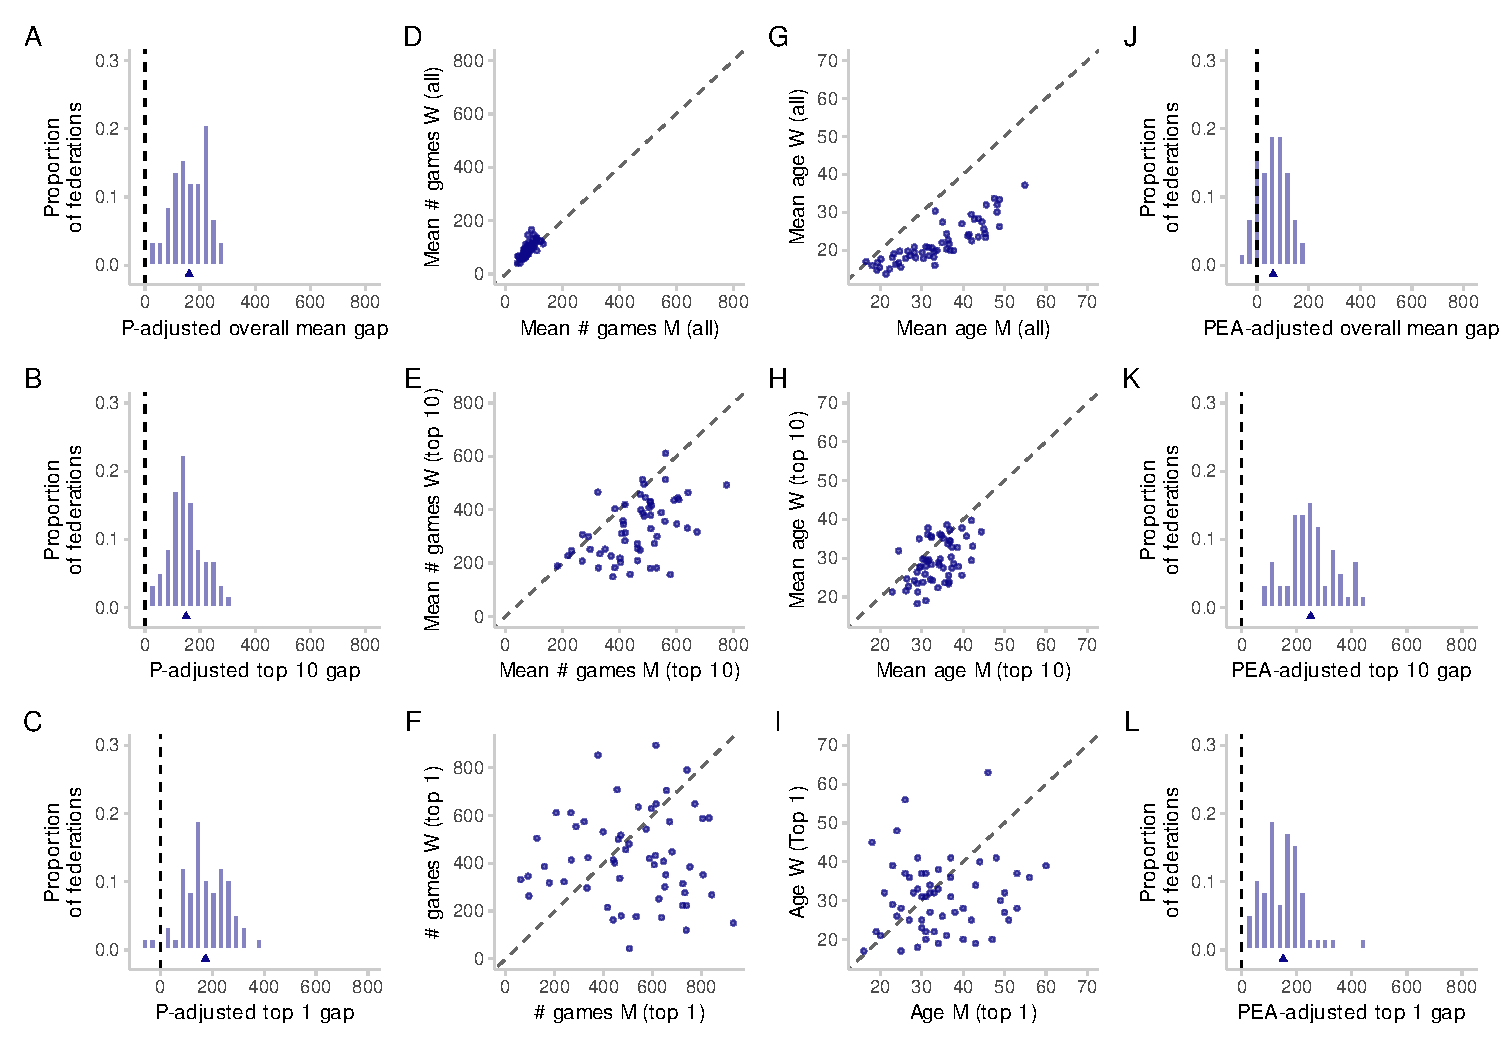
\includegraphics[width = \linewidth]{../figures/age-exp-juniors-noinactives-1400.pdf}
  \caption{As Fig.~3 in the main text, but with a rating floor of 1400 (sample size in each panel: 58).}
  \label{fig:age-exp-juniors-noinactives-1400}
\end{figure*}

\begin{figure*}[p]
  \centering
  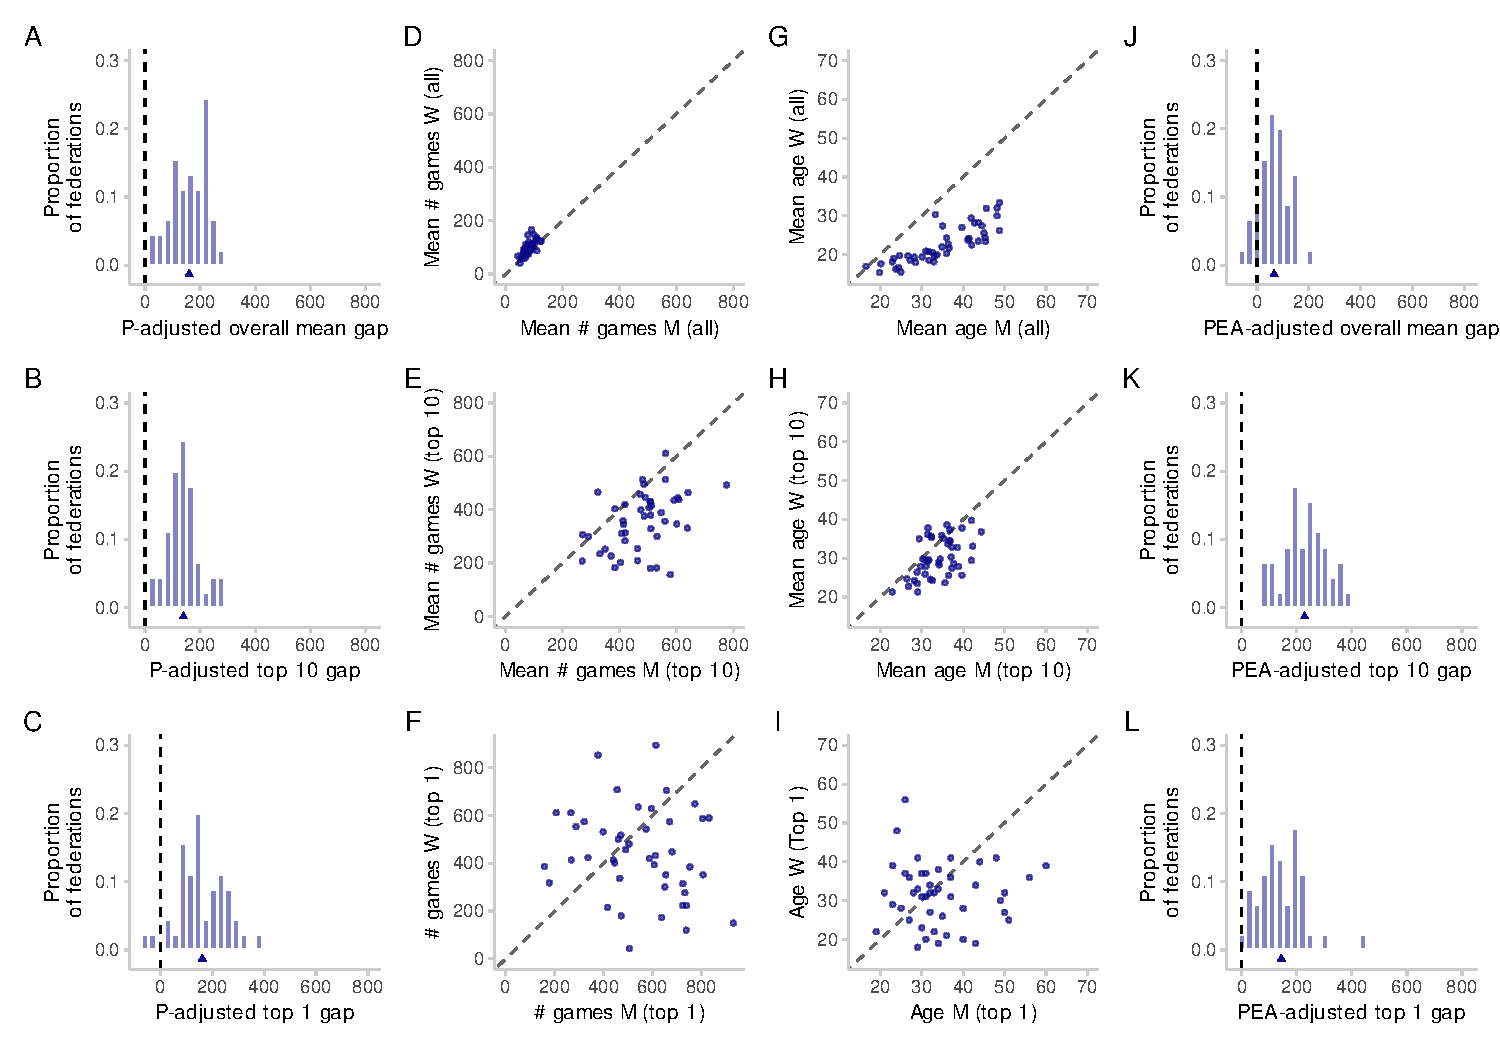
\includegraphics[width = \linewidth]{../figures/age-exp-juniors-noinactives-1600.pdf}
  \caption{As Fig.~3 in the main text, but with a rating floor of 1600 (sample size in each panel: 45).}
  \label{fig:age-exp-juniors-noinactives-1600}
\end{figure*}

\begin{figure*}[p]
  \centering
  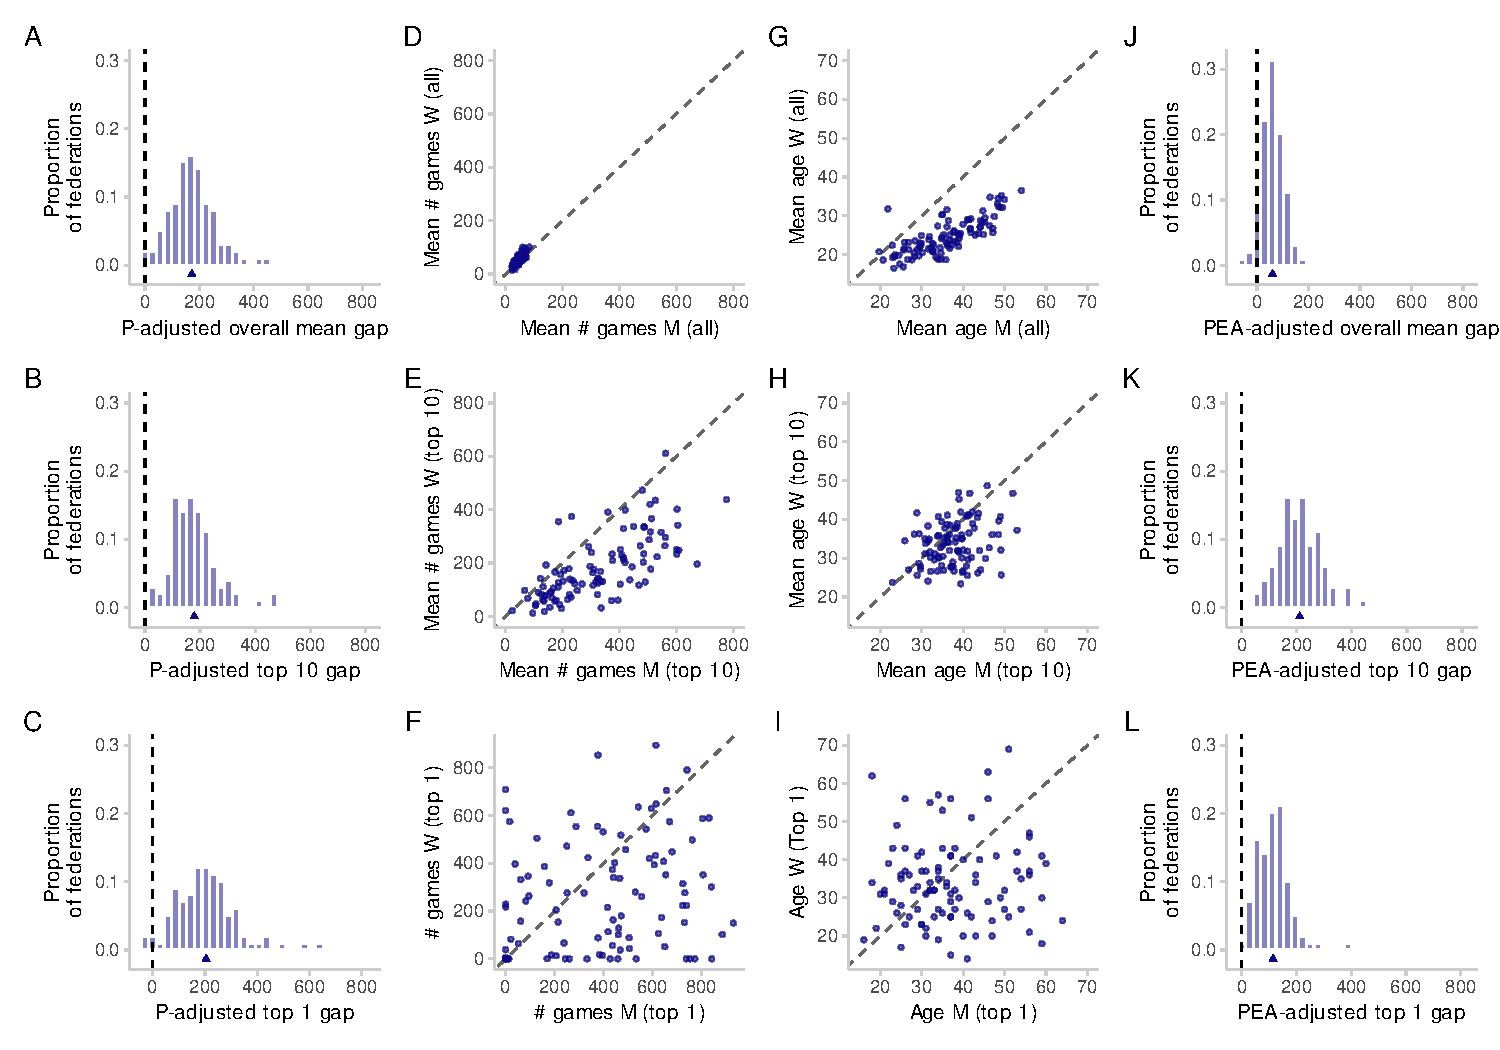
\includegraphics[width = \linewidth]{../figures/age-exp-juniors-inactives-1000.pdf}
  \caption{As Fig.~3 in the main text, but with both junior and inactive players, and a rating floor of 1000 (sample size in each panel: 99).}
  \label{fig:age-exp-juniors-inactives-1000}
\end{figure*}

\begin{figure*}[p]
  \centering
  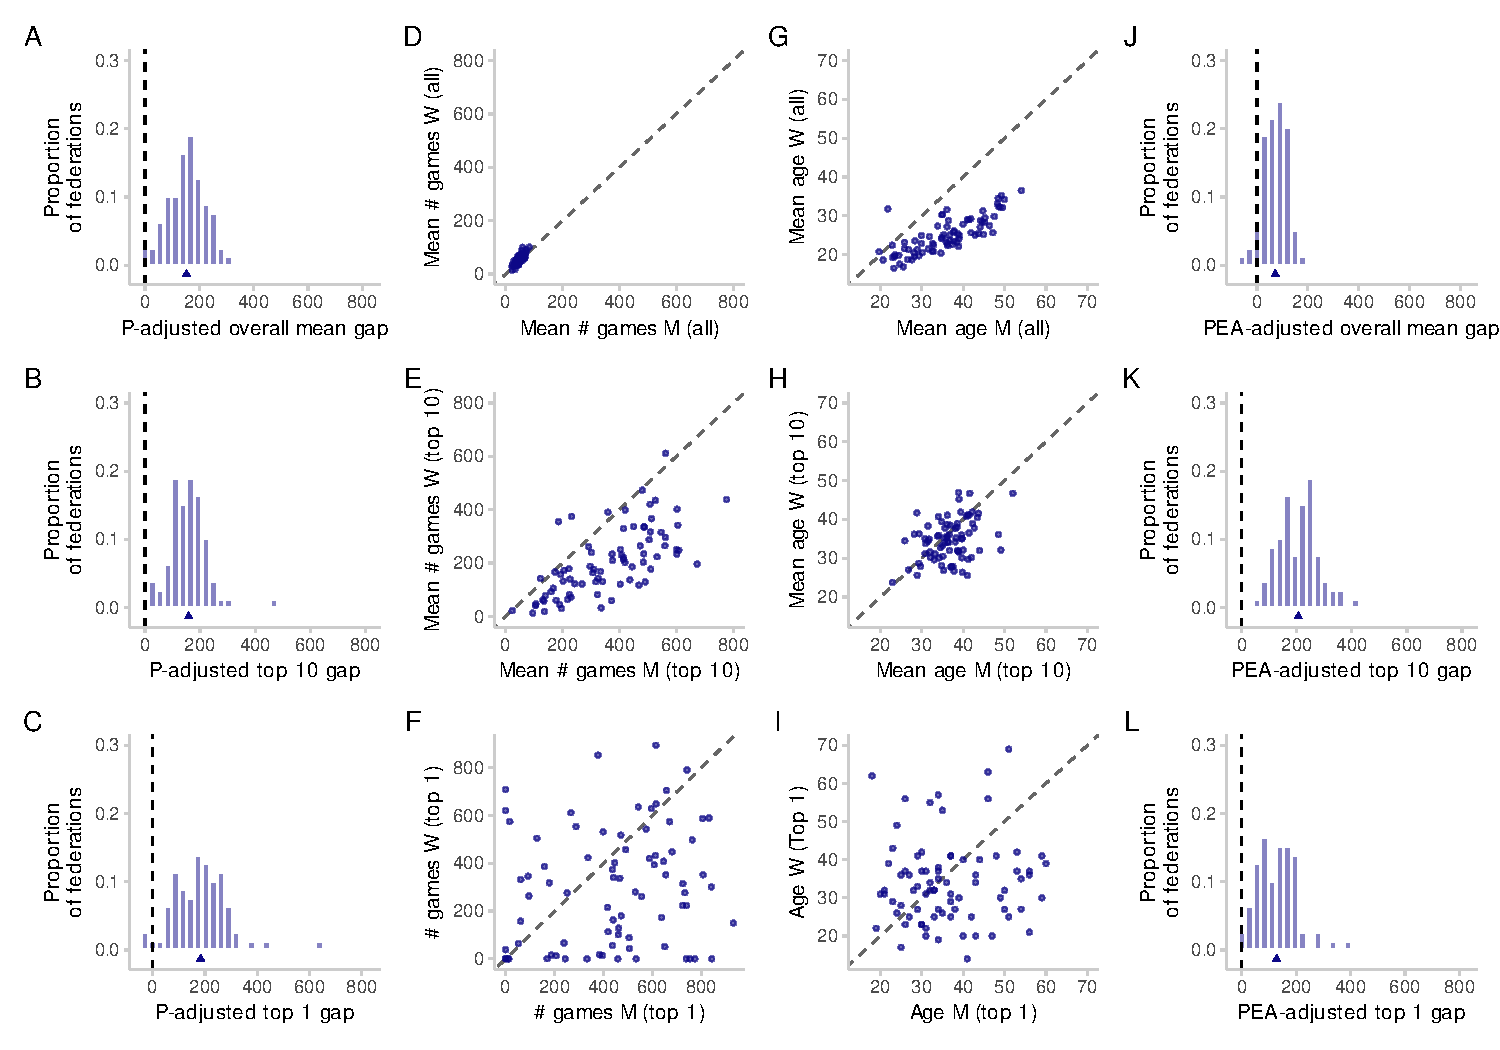
\includegraphics[width = \linewidth]{../figures/age-exp-juniors-inactives-1400.pdf}
  \caption{As Fig.~3 in the main text, but with both junior and inactive players, and a rating floor of 1400 (sample size in each panel: 79).}
  \label{fig:age-exp-juniors-inactives-1400}
\end{figure*}

\begin{figure*}[p]
  \centering
  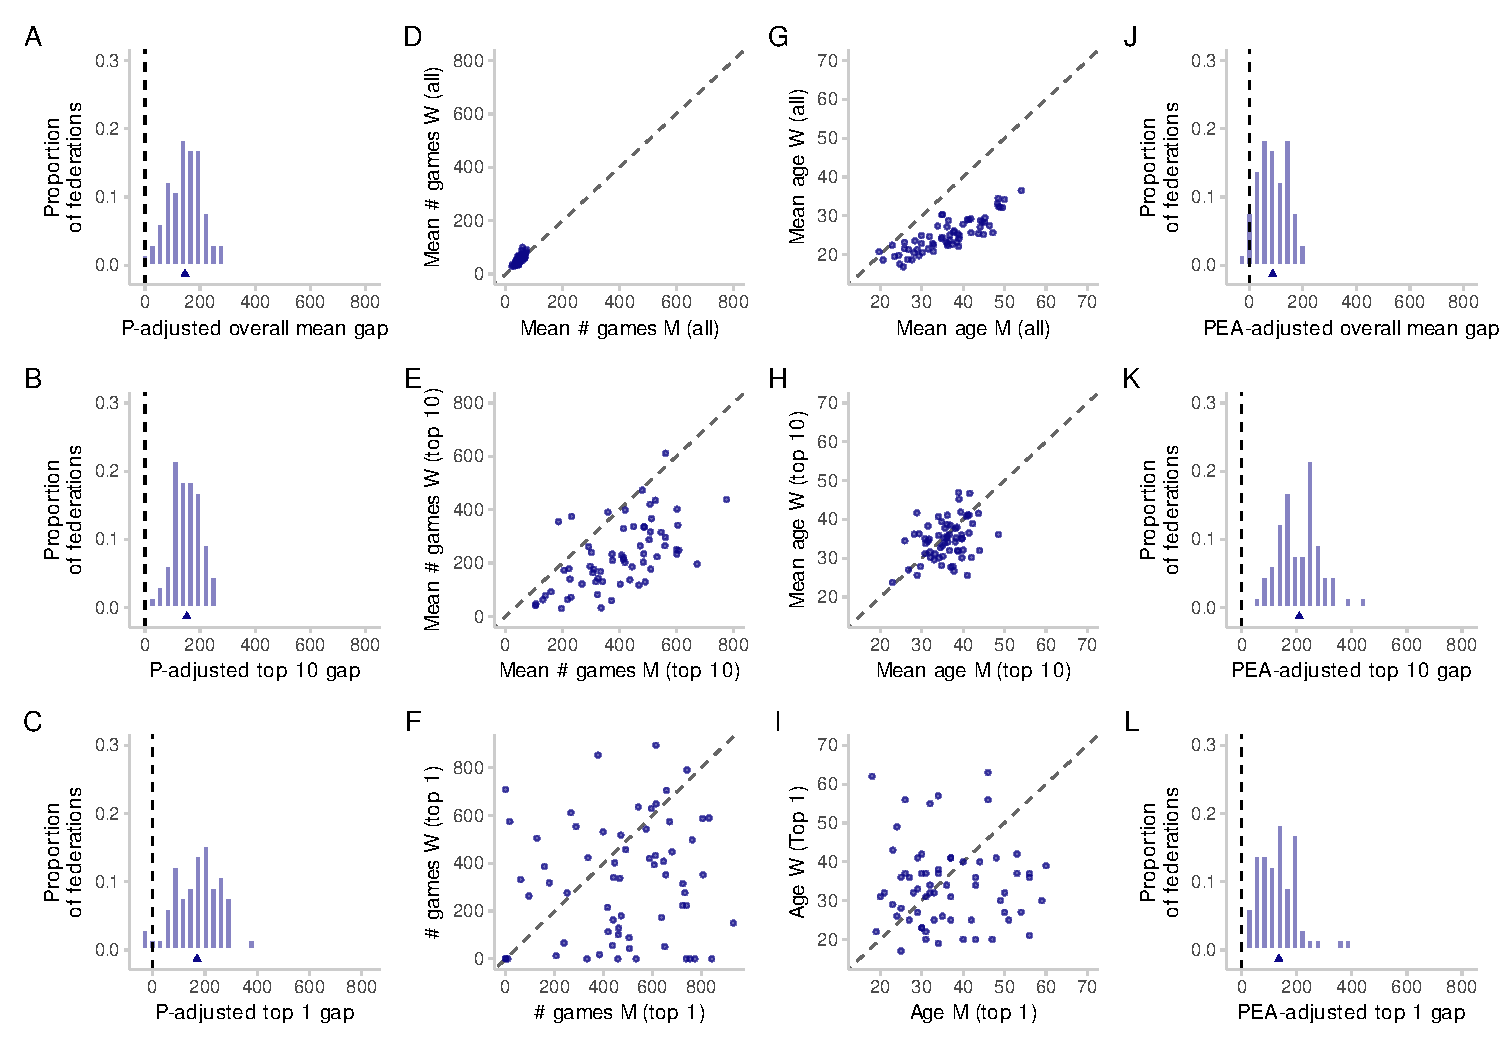
\includegraphics[width = \linewidth]{../figures/age-exp-juniors-inactives-1600.pdf}
  \caption{As Fig.~3 in the main text, but with both junior and inactive players, and a rating floor of 1600 (sample size in each panel: 65).}
  \label{fig:age-exp-juniors-inactives-1600}
\end{figure*}

\begin{figure*}[p]
  \centering
  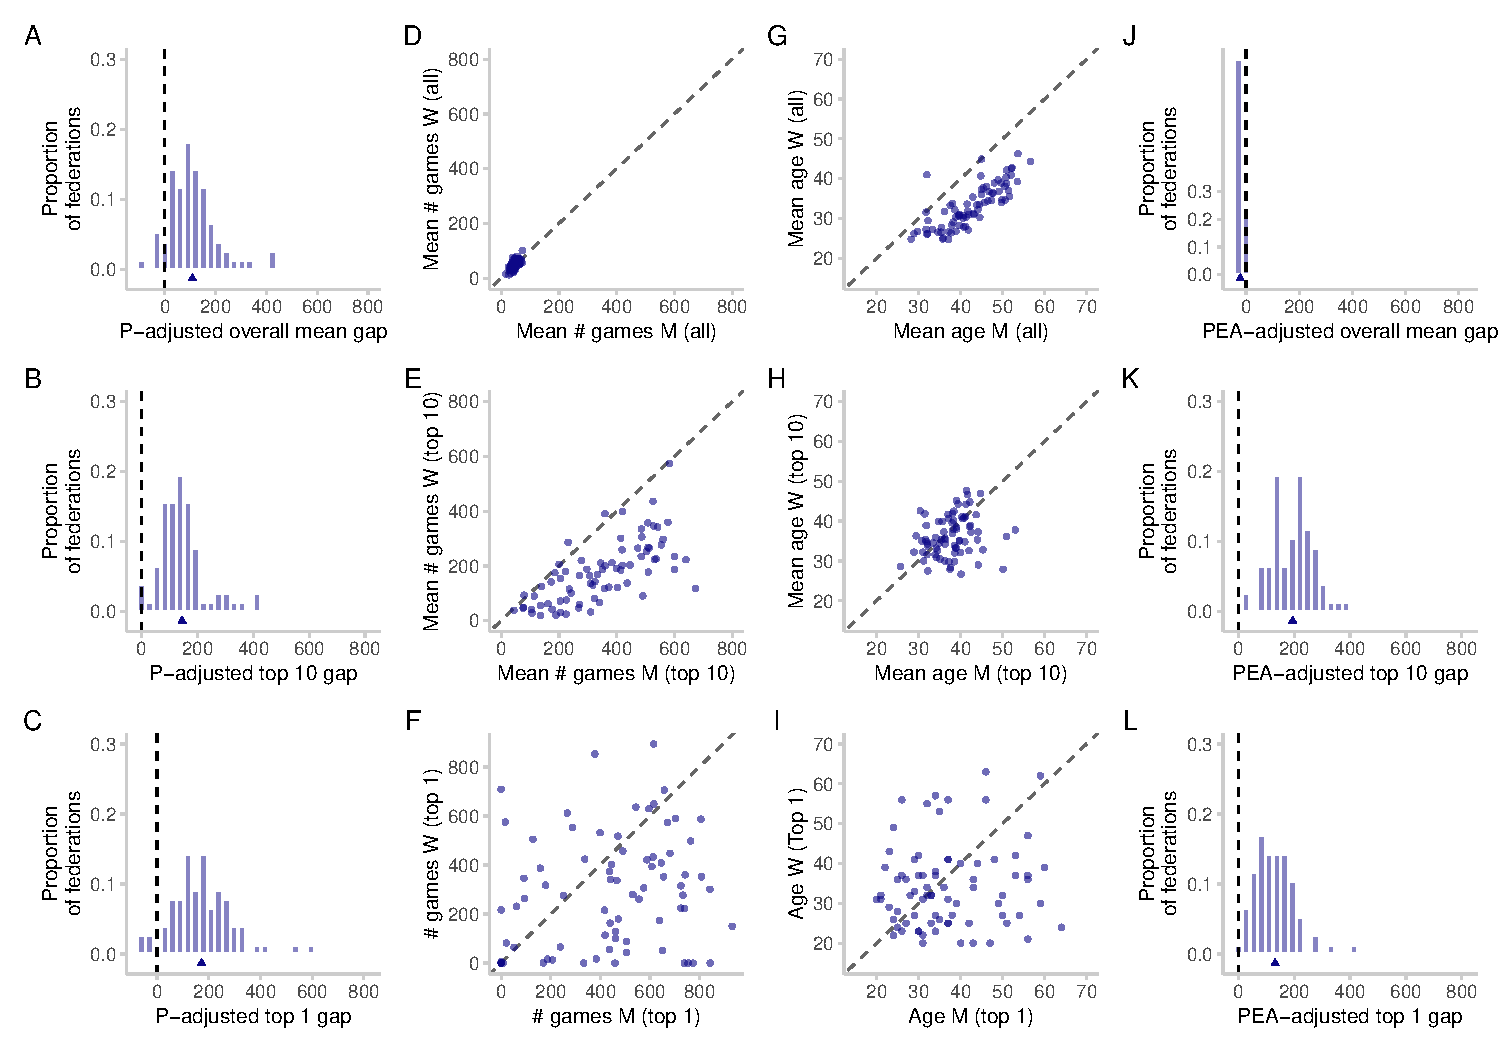
\includegraphics[width = \linewidth]{../figures/age-exp-nojuniors-inactives-1000.pdf}
  \caption{As Fig.~3 in the main text, but without junior and with inactive players, and a rating floor of 1000 (sample size in each panel: 77).}
  \label{fig:age-exp-nojuniors-inactives-1000}
\end{figure*}

\begin{figure*}[p]
  \centering
  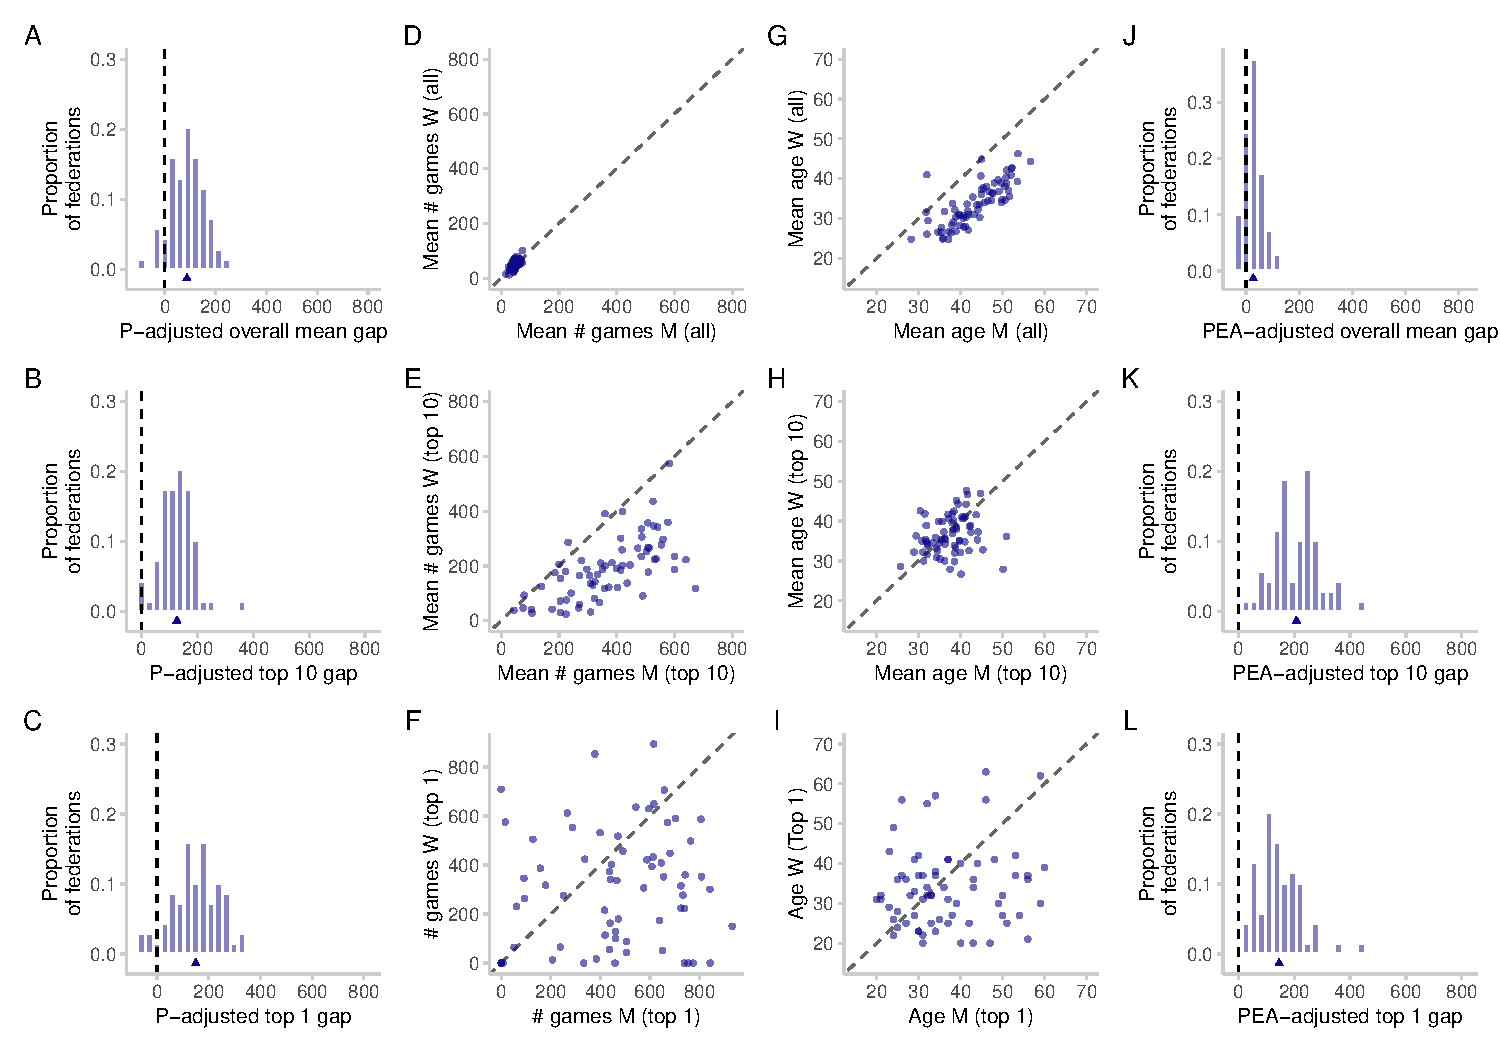
\includegraphics[width = \linewidth]{../figures/age-exp-nojuniors-inactives-1400.pdf}
  \caption{As Fig.~3 in the main text, but without junior and with inactive players, and a rating floor of 1400 (sample size in each panel: 69).}
  \label{fig:age-exp-nojuniors-inactives-1400}
\end{figure*}

\begin{figure*}[p]
  \centering
  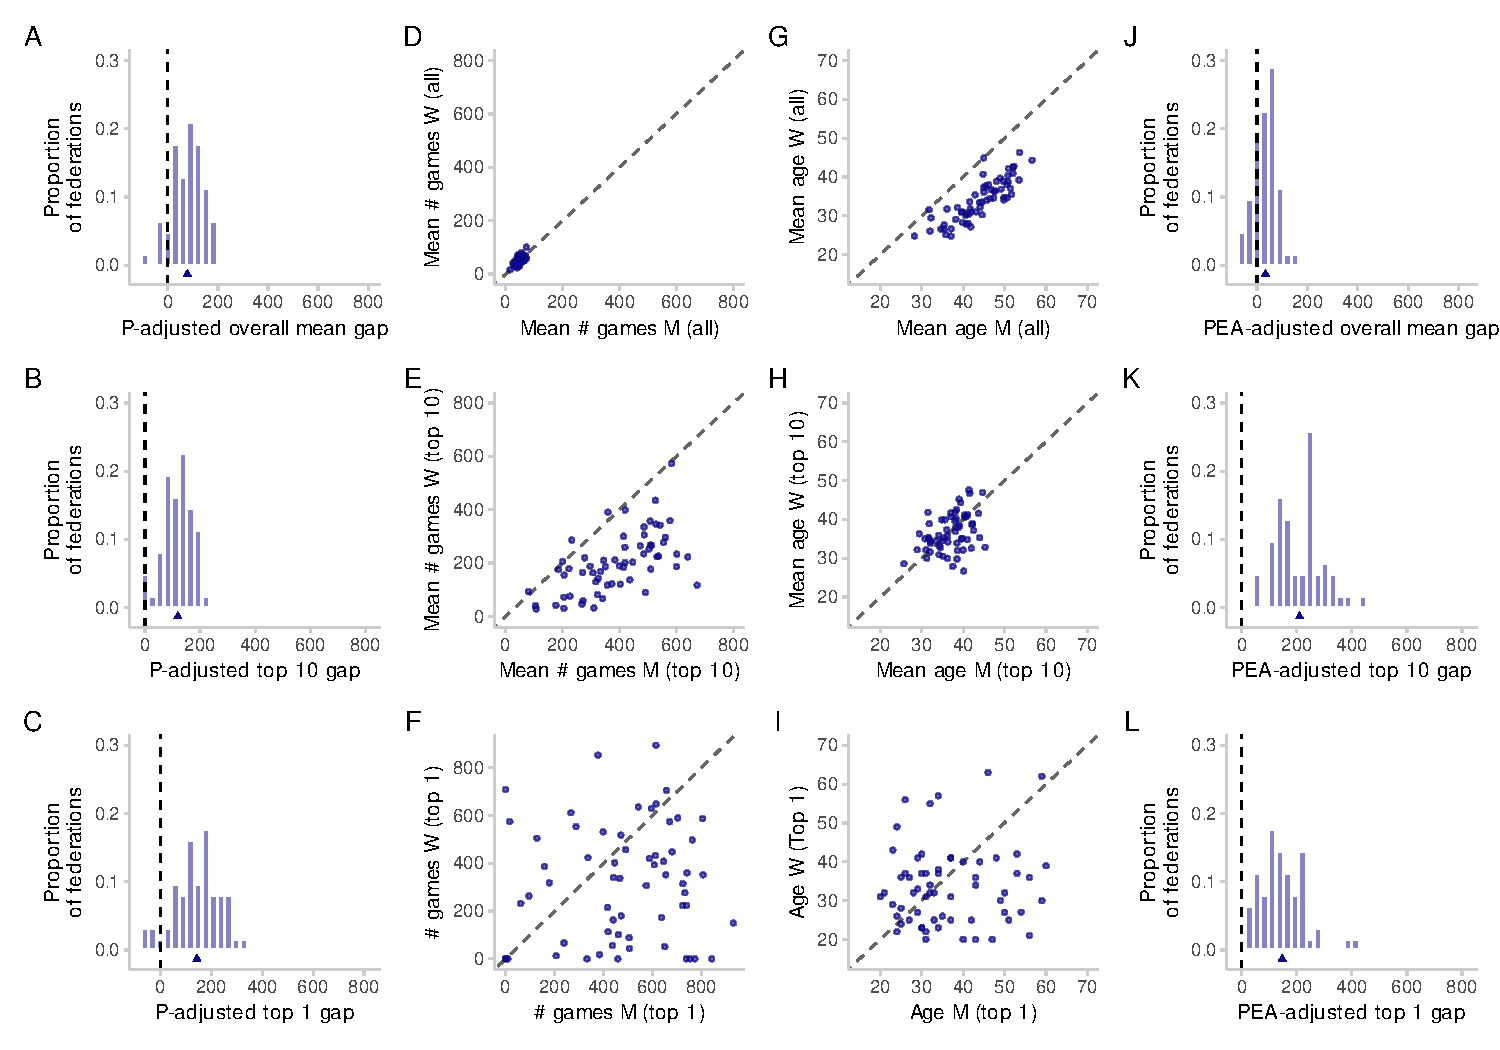
\includegraphics[width = \linewidth]{../figures/age-exp-nojuniors-inactives-1600.pdf}
  \caption{As Fig.~3 in the main text, but without junior and with inactive players, and a rating floor of 1600 (sample size in each panel: 62).}
  \label{fig:age-exp-nojuniors-inactives-1600}
\end{figure*}

\begin{figure*}[p]
  \centering
  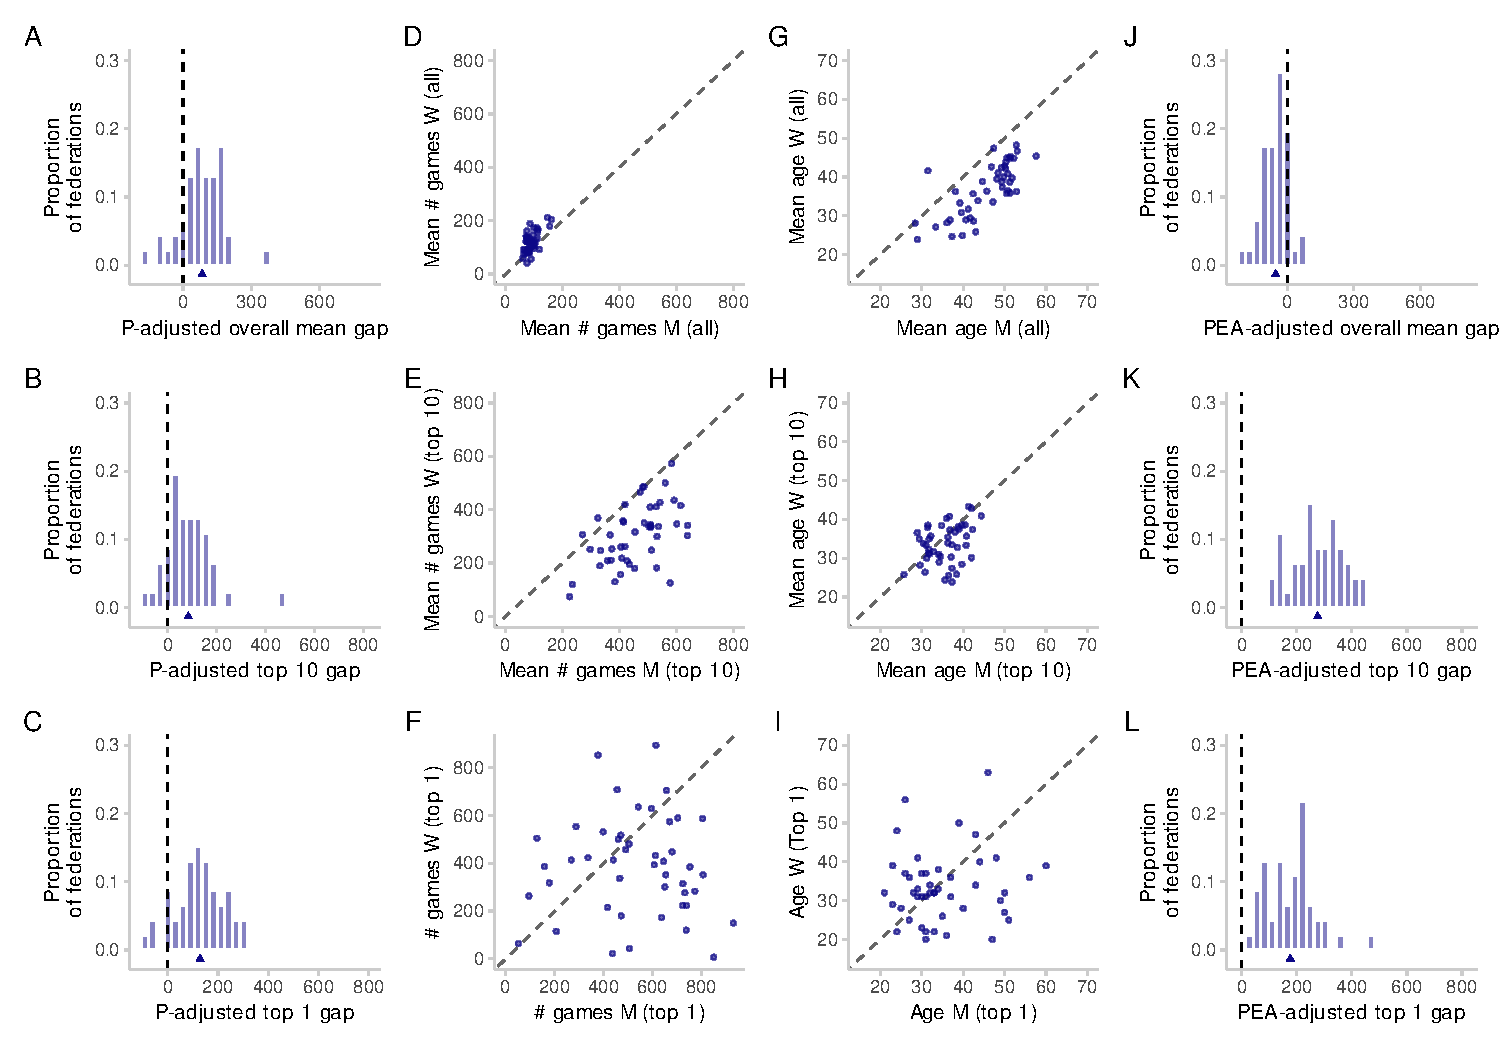
\includegraphics[width = \linewidth]{../figures/age-exp-nojuniors-noinactives-1000.pdf}
  \caption{As Fig.~3 in the main text, but without junior and without inactive players, and a rating floor of 1000 (sample size in each panel: 46).}
  \label{fig:age-exp-nojuniors-noinactives-1000}
\end{figure*}

\begin{figure*}[p]
  \centering
  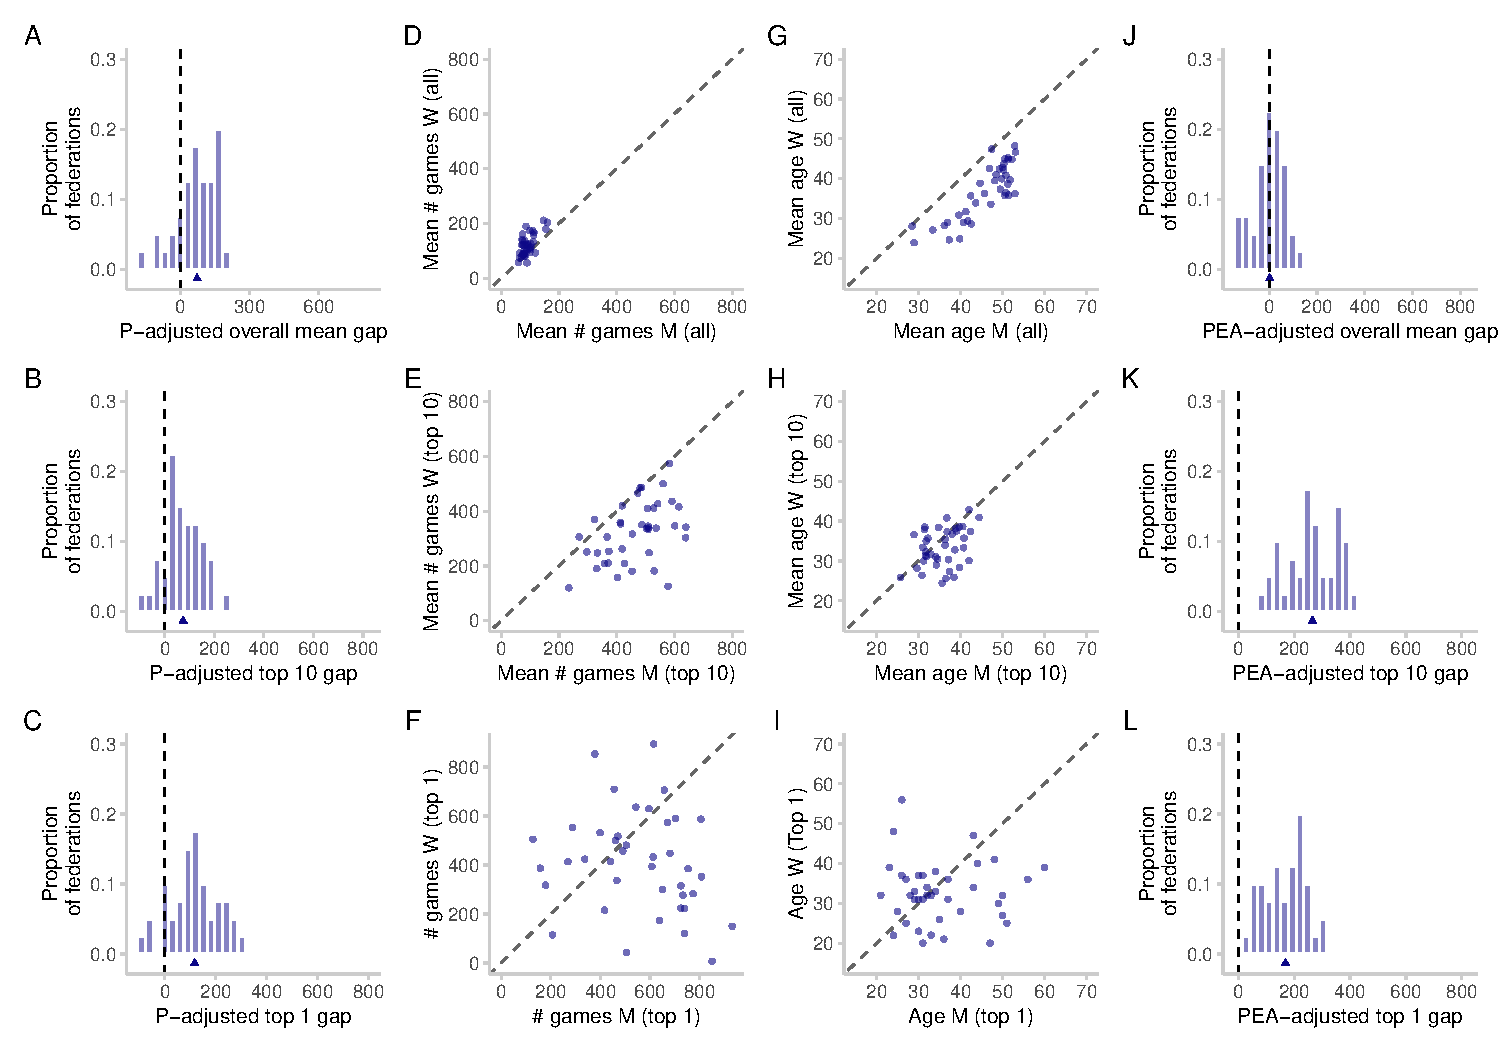
\includegraphics[width = \linewidth]{../figures/age-exp-nojuniors-noinactives-1400.pdf}
  \caption{As Fig.~3 in the main text, but without junior and without inactive players, and a rating floor of 1400 (sample size in each panel: 40).}
  \label{fig:age-exp-nojuniors-noinactives-1400}
\end{figure*}

\begin{figure*}[p]
  \centering
  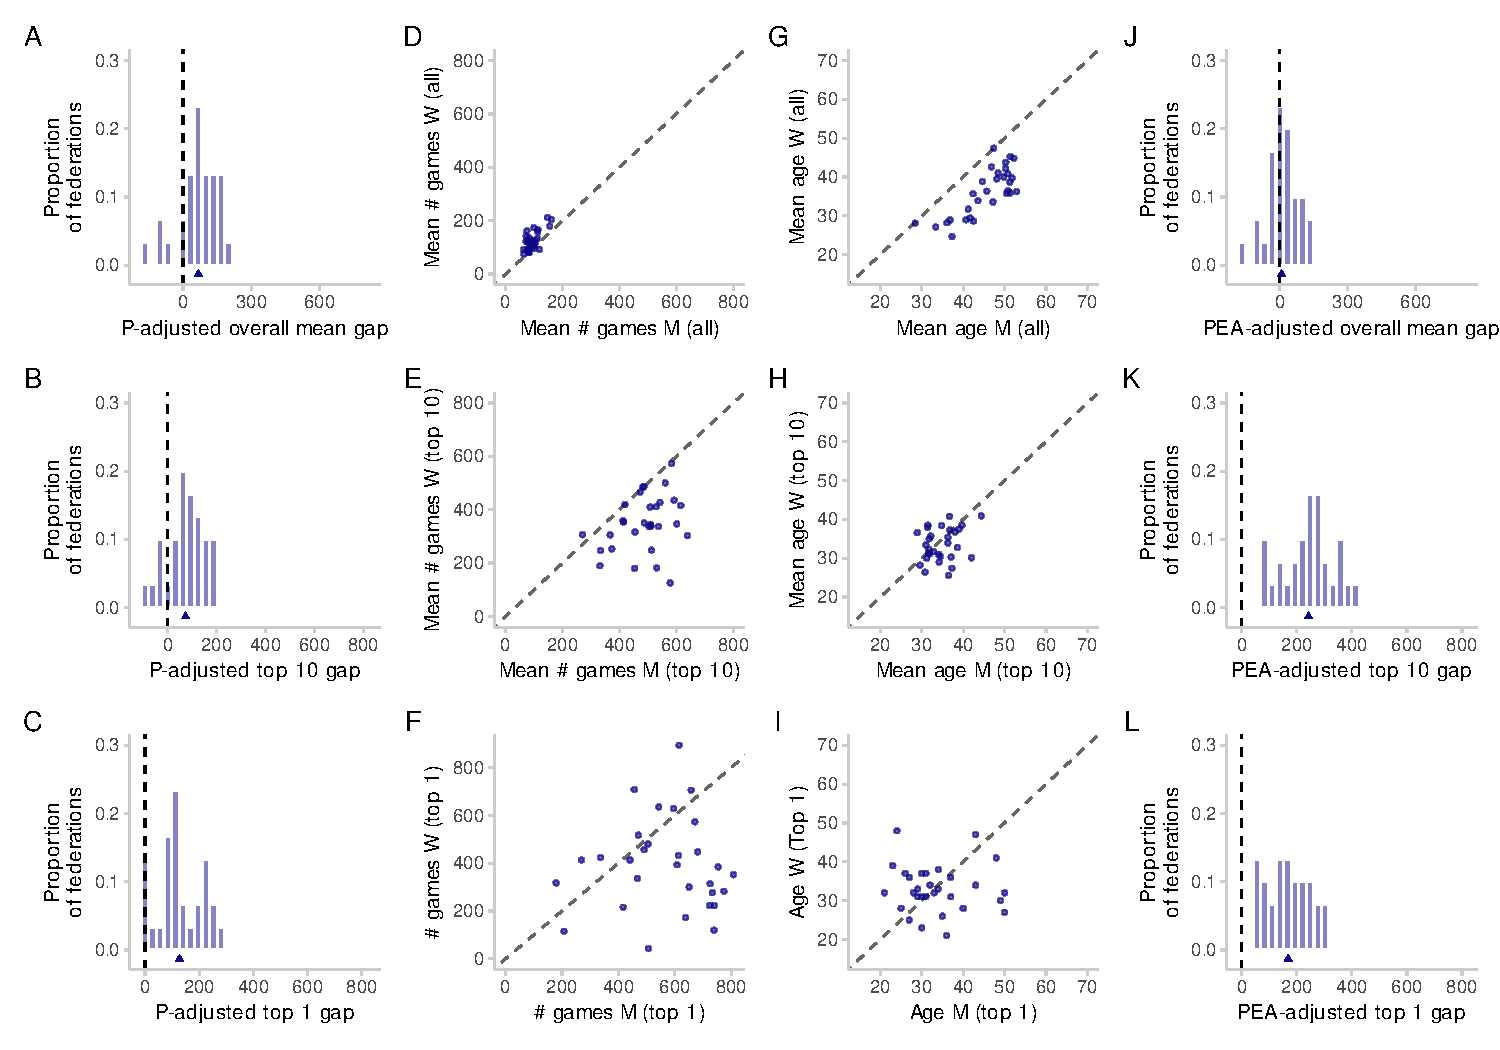
\includegraphics[width = \linewidth]{../figures/age-exp-nojuniors-noinactives-1600.pdf}
  \caption{As Fig.~3 in the main text, but without junior and without inactive players, and a rating floor of 1600 (sample size in each panel: 30).}
  \label{fig:age-exp-nojuniors-noinactives-1600}
\end{figure*}



%%% Add this line AFTER all your figures and tables
\FloatBarrier


\bibliography{references}


\end{document}

